\section{Query Processing and Optimization}

\subsection{What is Query Optimization?}

Query optimization is the act of reducing the runtime of queries in your database. This may be done through database design, indexes, query restructuring, or through hardware optimizations. It has become a topic that it is necessary to learn in today's world as in our data-driven society, it is imperative we are able to analyze data quickly and efficiently in the shortest time possible. Through query optimization, we can reduce runtime of queries from hours to mere minutes or even seconds. It is a concept that is important since as our world continues to collect more data, it is our job to make sure that we are able to use it and turn it into valuable information as quickly as possible.

\subsection{Query Optimization Strategies}

\subsubsection{Database Design and Normalization}

Proper database design and normalization play a major role in designing an OLAP application, as both the star and snowflake schemas have their own advantages and disadvantages. In a star schema, tables are denormalized, meaning that data is stored in a more straightforward and flattened structure. This design allows for faster query performance since fewer joins are required, but it can lead to increased storage requirements. On the other hand, the snowflake schema is normalized, meaning that there are much more tables that are stored to encourage joins, thus reducing the query runtime. However the benefit of this is that it uses far less storage compared to a star schema, making it beneficial as data warehouses are known to have large amounts of data that exceeds gigabytes of storage. For the purposes of our OLAP application, we had used the third type of schema, the starflake schema, in which only certain tables are normalized as it balances the storage and performance of queries, bringing out the best of both worlds \cite{ibm2021datawarehouse,kimball2013datawarehouse}. \\

As aforementioned, there are concepts within the database such as genre which has a very limited domain, which makes it rather unjustifiable to have its own table, rather than having to store 3 genre IDs that still have to be connected and joined to a different table. Decisions such as this are important to be captured through data profiling in order to make informed decisions to optimize the database even further. \\

\begin{figure}[H]
    \centering
    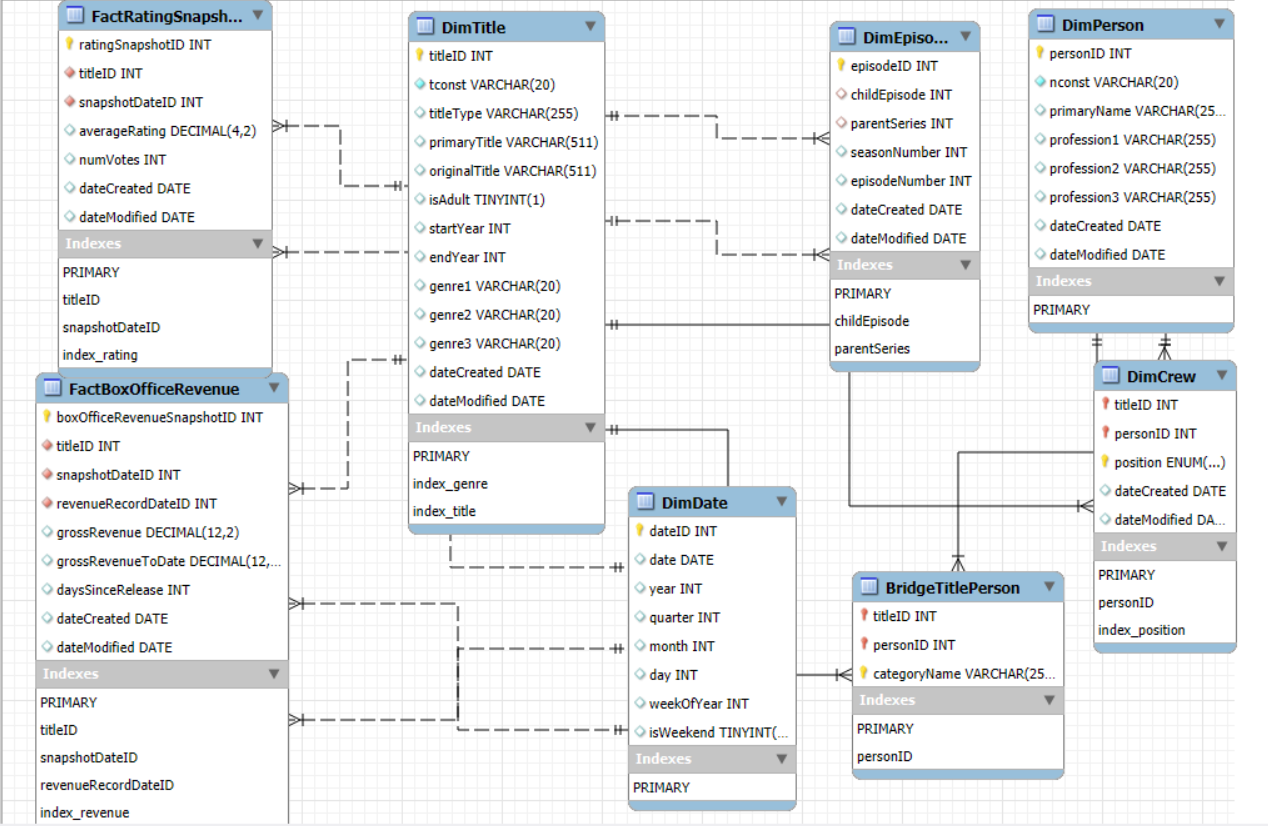
\includegraphics[width=0.8\linewidth]{images/schema.png}
    \caption{Schema for the OLAP Application}
    \label{fig:your_label}
\end{figure}

\subsubsection{Indexes}

Indexes are used in order to query results efficiently and is an essential tool in improving query performance. In the purposes of our OLAP application that analyzes rating, revenue, and genres, it was imperative that we create secondary indexes on these columns to decrease the runtime significantly. 

\begin{lstlisting}
CREATE INDEX index_position
ON DimCrew (position)

CREATE INDEX index_genre
ON DimTitle (genre1, genre2, genre3)

CREATE INDEX index_title
ON DimTitle (titleType)

CREATE INDEX index_rating
ON FactRatingSnapshot (averageRating)

CREATE INDEX index_revenue
ON FactBoxOfficeRevenue (grossRevenueToDate)
\end{lstlisting}

\subsubsection{Query Restructuring}

The queries we had used in our application had numerous optimizations, restructuring, and formatting for readability. CTEs were used throughout majority of the queries for formatting alongside the inner queries being the most selective to return the least amount of rows as possible. Doing this decreases the query runtime and allows us to retrieve thousands to tens of thousands in a sea of tens of millions of rows in mere seconds. Additionally, operations such as only selecting required columns, aggregates and early filtering proved to be effective in further decreasing the runtime to strive for the most optimized query runtime as possible.

\begin{lstlisting}
WITH Movies(titleID) AS ( 
        SELECT dt.titleID
        FROM DimTitle dt
        WHERE dt.titleType = 'movie'
    )
SELECT 
    SUM(fbor.grossRevenue) / 1000000 
        AS totalRevenueThatDayInMillions, 
    dd.year, 
    dd.month, 
    dd.day
FROM Movies m
JOIN FactBoxOfficeRevenue fbor 
ON fbor.titleID = m.titleID
JOIN DimDate dd 
ON dd.dateID = fbor.revenueRecordDateID
WHERE dd.year = "2024"
GROUP BY dd.year, dd.month, dd.day
ORDER BY dd.year, dd.month, dd.day;
\end{lstlisting}

Such example shows that the table for Movies is much more readable since it is contained in the CTE rather than being  stored in a subquery.

\subsubsection{Optimization at Hardware Level}

Alongside database design, indexes, and query restructuring, providing an appropriate amount of hardware resources is another important point of focus as the CPU, RAM, and storage are important aspects of querying operations. The database server contains 4 cores, 12GB of RAM, and 64GB of disk storage to store the entire IMDB dataset.